\documentclass[12pt]{article}
\usepackage[T1]{fontenc}
\usepackage{tkz-tab}

\begin{document}

\raggedright
$\textbf{Pour~} \mathbf{\Delta} \textbf{> 0 on a :}$
\begin{center}
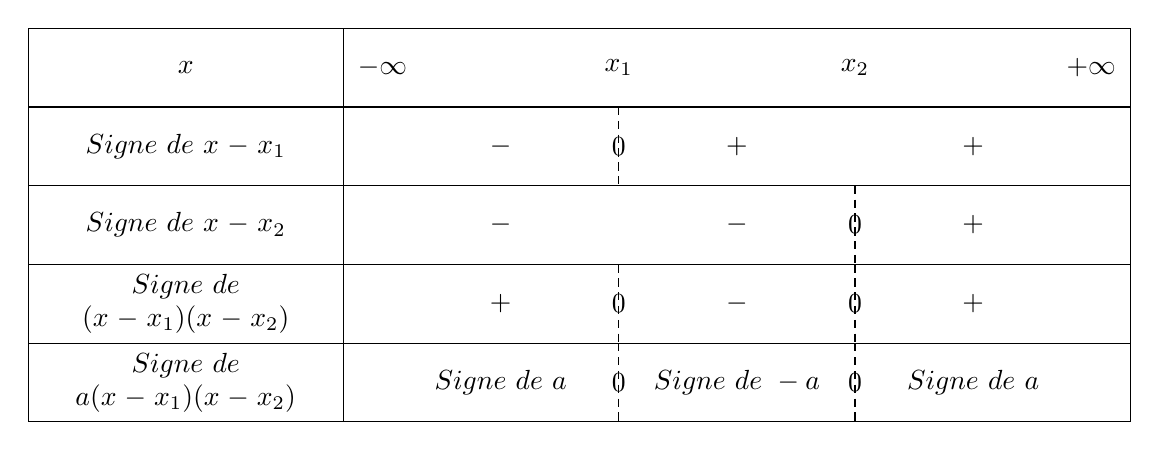
\begin{tikzpicture}
\tikzset{t style/.style = {style = densely dashed}}
\tkzTabInit[color,lgt=4,espcl=3]%
{$x$/1,$Signe~de~x-x_1$/1,$Signe~de~x-x_2$/1,$Signe~de$\\
$(x-x_1)(x-x_2)$/1,$Signe~de$\\
$a(x-x_1)(x-x_2)$/1}{$-\infty$,$x_1$,$x_2$,$+\infty$}%
\tkzTabLine{, -,z,+, ,+}
\tkzTabLine{, -, , -, z,+}
\tkzTabLine{, +, z, -, z,+}
\tkzTabLine{, Signe~de~a, z, Signe~de~-a, z,Signe~de~a}
\end{tikzpicture}
\end{center}

$\textit{On dit que le pôlynome est du signe de a à l'extérieur des racines.}$\\[30pt]

\raggedright
$\textbf{Pour~} \mathbf{\Delta} \textbf{= 0 on a :}$

\begin{center}
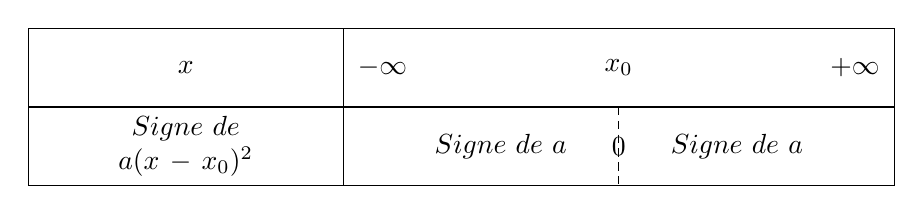
\begin{tikzpicture}
\tikzset{t style/.style = {style = densely dashed}}
\tkzTabInit[lgt=4,espcl=3]%
{$x$/1,$Signe~de$\\
$a(x-x_0)^2$/1}{$-\infty$,$x_0$,$+\infty$}%
\tkzTabLine{, Signe~de~a,z,Signe~de~a,}
\end{tikzpicture}
\end{center}

\raggedright
$\textbf{Pour~} \mathbf{\Delta} \textbf{< 0 on a :}$

\begin{center}
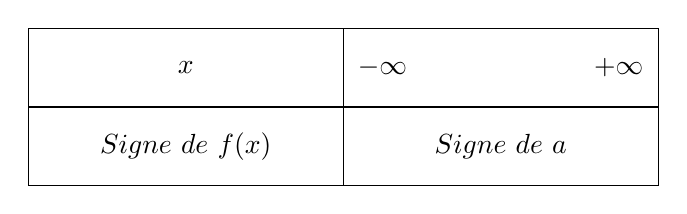
\begin{tikzpicture}
\tikzset{t style/.style = {style = densely dashed}}
\tkzTabInit[lgt=4,espcl=3]%
{$x$/1,$Signe~de~f(x)$/1}{$-\infty$,$+\infty$}%
\tkzTabLine{, Signe~de~a,}
\end{tikzpicture}
\end{center}

\end{document}